\documentclass{article}
\usepackage{bm}
\usepackage{amsmath}
\usepackage{graphicx}
\usepackage{mdwlist}
\usepackage[colorlinks=true]{hyperref}
\usepackage{geometry}
\usepackage{kotex}
\geometry{margin=1in}
\geometry{headheight=2in}
\geometry{top=2in}
\usepackage{palatino}
%\renewcommand{\rmdefault}{palatino}
\usepackage{fancyhdr}

%\pagestyle{fancy}
\rhead{}
\lhead{}
\chead{%
  {\vbox{%
      \vspace{2mm}
      \large
      Hardware System Design 4190.309A\hfill
\\
      Seoul National University
      \\[4mm]
      \textbf{Practice \#5. PE implementation \& BRAM modeling}\\
      \textbf{Jiwon Lee, Sangjun Son}
    }
  }
}

%%%%%%%%%%%%%%%%%%%%%%%
\usepackage{xcolor}
\usepackage{listings}
\definecolor{vgreen}{RGB}{104,180,104}
\definecolor{vblue}{RGB}{49,49,255}
\definecolor{vorange}{RGB}{255,143,102}

\lstdefinestyle{verilog-style}
{
    language=Verilog,
    basicstyle=\scriptsize\ttfamily,
    keywordstyle=\color{vblue},
    identifierstyle=\color{black},
    commentstyle=\color{vgreen},
    numbers=left,
    numberstyle=\tiny\color{black},
    numbersep=10pt,
    tabsize=8,
    moredelim=*[s][\colorIndex]{[}{]},
    literate=*{:}{:}1
}

\makeatletter
\newcommand*\@lbracket{[}
\newcommand*\@rbracket{]}
\newcommand*\@colon{:}
\newcommand*\colorIndex{%
    \edef\@temp{\the\lst@token}%
    \ifx\@temp\@lbracket \color{black}%
    \else\ifx\@temp\@rbracket \color{black}%
    \else\ifx\@temp\@colon \color{black}%
    \else \color{vorange}%
    \fi\fi\fi
}
\makeatother

\usepackage{trace}
%%%%%%%%%%%%%%%%%%%%%%%

\usepackage{paralist}

\usepackage{todonotes}
\setlength{\marginparwidth}{2.15cm}

\usepackage{tikz}
\usetikzlibrary{positioning,shapes,backgrounds}

\begin{document}

\pagestyle{fancy}

\section*{Goal}

\begin{itemize*}
\item Implement BRAM model \& test bench according to scenarios.
\begin{itemize*}
\item Make test bench that instantiates two BRAMs and initialize one BRAM to store address as data.
\item Copy every data from the initialized BRAM to the other BRAM.
\end{itemize*}
\item Implement PE with floating point fused multiply adder.
\end{itemize*}

\section{Implementation}

이번 프로젝트는 Block Random Access Memory와 Processing Element를 각각 구현함으로써 추후 구현할 Matrix-Matrix Multiplication을 수행하기 위한 기본 모듈을 구성하는 것을 목적으로 한다. 아래는 코드 구현과 함께 간략한 아이디어 및 기능에 대한 설명이 (1) BRAM, (2) PE 순으로 진행된다.

\subsection{Block Random Access Memory, BRAM}
BRAM의 경우 크게 두 부분으로 이뤄져 있다. (1) 모듈이 실행이 되기 전 INIT\_FILE에서 내부 메모리 \texttt{mem}를 읽는 부분과 done 신호가 주어졌을 때, OUT\_FILE에 \texttt{mem}의 상태를 출력하는 부분과, (2) EN, RST, WE 신호가 들어왔을 때 경우에 따라 입력되는 데이터를 \texttt{mem}에 읽고 쓰는 역할을 한다.

\begin{itemize*}
\item 아래에 첨부된 코드 중 21-28 라인의 외부 파일 입출력에 관한 구현 보면, \texttt{initial} 구문을 이용하여 모듈의 생성과 동시에 파일 입출력에 대한 실행 구문에 대한 scope를 지정한다. 
\texttt{\$readmemh} 로 시작함으로써 INIT\_FILE 파일을 읽어 \texttt{mem}에 저장한다. 
그 후 \texttt{done} 신호 들어올 때 까지 대기하다가 신호가 들어오면 \texttt{\$writememh} 함수를 사용해 OUT\_FILE에 \texttt{mem} 데이터를 저장한다.
이 때 함수에 붙어있는 \texttt{\$readmem\textbf{h}}와 \texttt{\$writemem\textbf{h}}의 \textbf{h}는 hexadecimal로 파일에 저장하는 값을 16진수 형태로 저장하는 옵션을 의미한다~\cite{memh}. \\
\item 30-46 라인은 BRAM의 input으로 주어지는 신호에 따라 모듈로써의 기능을 구현하는 부분이다. BRAM\_CLK와 BRAM\_RST 그리고 BRAM\_EN, BRAM\_WE의 신호에 따라 읽기, 쓰기, 초기화, 파일 출력을 위한 기능을 수행하게 된다. BRAM\_RST은 BRAM\_CLK에 Async로, BRAM\_EN, BRAM\_WE는 Sync로 구현하였다.
\begin{itemize*}
\item BRAM\_RST이 posedge일 경우 BRAM\_RDDATA에는 0을 할당한다. (31 라인)
\item BRAM\_EN이 활성화되어 있고 BRAM\_WE 또한 활성화되어 있다면, True를 가지는 bit에 해당하는 영역을 BRAM\_WRDATA에서 \texttt{mem}으로 복사한다. (35-38 라인)
\begin{equation}
\texttt{mem}[ \texttt{addr} ][8*(i+1)-1:8* i ]  \leftarrow \text{BRAM\_WRDATA}[8*(i+1) -1:8* i ] 
\end{equation}
\item BRAM\_EN이 활성화되어 있고 BRAM\_WE이 활성화되어 있다면, 메모리로부터 데이터를 읽어오는 기능을 수행한다. Read에 걸리는 싸이클이 2 cycle이 걸리도록 구현을 해야하기 때문에 \texttt{dout}을 버퍼로 사용해 1 cycle이 추가되도록 한다. (41-42 라인)
\end{itemize*}
\end{itemize*}

\newpage
\subsubsection*{\texttt{MY\_BRAM}}
\begin{lstlisting}[style={verilog-style}]
`timescale 1ns / 1ps
module my_bram #(
    parameter integer BRAM_ADDR_WIDTH = 15,
    parameter INIT_FILE = "input.txt",
    parameter OUT_FILE = "output.txt"
)(
    input wire [BRAM_ADDR_WIDTH-1:0] BRAM_ADDR,
    input wire BRAM_CLK,
    input wire [31:0] BRAM_WRDATA,
    output reg [31:0] BRAM_RDDATA,
    input wire BRAM_EN,
    input wire BRAM_RST,
    input wire [3:0] BRAM_WE,
    input wire done
);
    reg [31:0] mem[0:8191];
    wire [BRAM_ADDR_WIDTH-3:0] addr = BRAM_ADDR[BRAM_ADDR_WIDTH-1:2];
    reg [31:0] dout;
    
    initial begin
        if (INIT_FILE != "") begin
            $readmemh(INIT_FILE, mem);
        end
        wait (done) begin
            $writememh(OUT_FILE, mem);
        end
    end
    
    always @(posedge BRAM_CLK or posedge BRAM_RST) begin
        if (BRAM_RST) begin 
            BRAM_RDDATA <= 0;
        end
        if (BRAM_EN) begin
            if (BRAM_WE) begin
                if (BRAM_WE[0]) mem[addr][7:0] <= BRAM_WRDATA[7:0];
                if (BRAM_WE[1]) mem[addr][15:8] <= BRAM_WRDATA[15:8];
                if (BRAM_WE[2]) mem[addr][23:16] <= BRAM_WRDATA[23:16];
                if (BRAM_WE[3]) mem[addr][31:24] <= BRAM_WRDATA[31:24]; 
            end
            else begin
                dout <= mem[addr];
                BRAM_RDDATA <= dout;
            end
        end
    end
endmodule
\end{lstlisting}

\quad
\subsection{Processing Element, PE}

Processing Element (이하 PE)는 구현의 최종목표인 CNN에서 벡터의 내적연산을 계산하는 역할을 한다. PE의 구현방식은 다음과 같다.
\begin{enumerate}
    \item 외부 컨트롤러 (현재는 testbench로 대체)에서 들어온 input값들을 받는다.
    \item ain, bin, cin로 floating point fused multiply-add(이하 MAC)를 수행한다.
    \item (2)에서 나온 결과값을 psum에 더해준다.
    \item (1),(2),(3)을 모든 입력값에 대해 반복해서 수행한다.
\end{enumerate}

위의 구현을 수식으로 나타내면 다음과 같다. 
\begin{equation*}
\texttt{psum} = \texttt{ain}_i \times \texttt{bin}_i + \texttt{psum  }(\texttt{i} : \texttt{input number}) 
\end{equation*}

MAC모듈의 parameter중 dvalid bit는 연산이 끝난 후, m\_axis\_result\_tdata가 실제 연산의 결과값임을 보장해준다. 따라서, always구문을 사용하여 결과값을 다시 psum register에 저장해 주었다. 코드를 보면, s\_axis\_c\_tdata과 m\_axis\_result\_tdata가 다름을 확인 할 수 있는데, 이는 MAC에서 parallel 하게 cin과 result값을 parameter로 줄 수 없기 때문이다. 따라서, 임시 res register를 이용하여 결과값을 받았고, 이후 그 값을 psum에 할당해주었다.

\subsubsection*{\texttt{MY\_PE}}
\begin{lstlisting}[style={verilog-style}]
`timescale 1ns / 1ps

module my_pe #(
    parameter L_RAM_SIZE = 6,
    parameter BITWIDTH = 32
)
(
    input aclk,
    input aresetn,
    input [BITWIDTH-1:0] ain,
    input [BITWIDTH-1:0] bin,
    input valid,
    output dvalid,
    output [BITWIDTH-1:0] dout
);

    // local reg ( can make overflow )
    reg [BITWIDTH-1:0] psum = 0;
    wire [BITWIDTH-1:0] res;
    
    floating_point_MAC UUT (
        .aclk(aclk),
        .aresetn(aresetn),
        .s_axis_a_tvalid(valid),
        .s_axis_b_tvalid(valid),
        .s_axis_c_tvalid(valid),
        .s_axis_a_tdata(ain),
        .s_axis_b_tdata(bin),
        .s_axis_c_tdata(psum),
        .m_axis_result_tvalid(dvalid), 
        .m_axis_result_tdata(res)
    );
  
    always @(dvalid) begin
        if(dvalid == 1) begin
            psum = res;
        end
    end
    
    assign dout = dvalid == 1 ? psum : 0;
endmodule
\end{lstlisting}

\newpage
\section{Result}

\subsection{Block Random Access Memory, BRAM}
아래의 코드는 BRAM의 구현의 Validity를 확인하기 위해 시나리오에 맞게 구현한 것이다. BRAM 인스턴스 두 개를 만들고 각각을 MY\_BRAM1과 MY\_BRAM2로 명명하였다. 

MY\_BRAM1은 \texttt{input.txt}에 저장된 \texttt{mem}에 있는 값들을 호출하여 저장하는 역할을 하고 또한 \texttt{mem}에 있는 값들을 MY\_ADDR을 변화하면서 BRAM\_RDDATA1로 읽어온다. MY\_BRAM2의 경우 이렇게 읽어온 \linebreak BRAM\_RDDATA1을 BRAM\_WRDATA2로 사용하여 \texttt{mem}에 저장하게 되고 완료가 되면 \texttt{done} 신호를 주어 \linebreak \texttt{output.txt}에 저장하게 된다. 아래 Figure~\ref{fig1}은 상기된 설명을 도식화한 것이다.
\begin{figure}[ht]
	\centering
	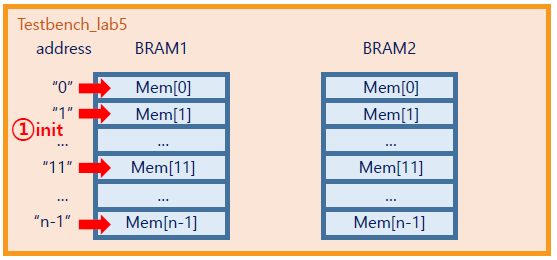
\includegraphics[width=0.49\textwidth]{fig/fig1.png}
	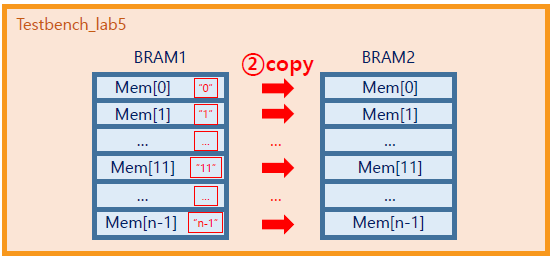
\includegraphics[width=0.49\textwidth]{fig/fig2.png}
\caption{Testbench Scenarios: 2개의 BRAM을 인스턴스화 하고 BRAM1에서 \texttt{input.txt}을 읽어 메모리에 저장하고 다른 BRAM2에서 BRAM1의 데이터를 전달받아  \texttt{output.txt}에 저장한다~\cite{lab}. }
\label{fig1}
\end{figure}
\begin{itemize*}
\item 모든 테스트를 시작하기 전에 \texttt{input.txt}를 초기화하기 위한 과정을 거친다. 주소에 해당하는 인덱스를 값으로 가질 수 있도록 for문을 통해 대입시킨 후 \texttt{\$writememh}를 통해 파일에 저장을 한다 (23-24 라인).\\
\item 테스트벤치에서 BRAM\_EN 신호는 항상 활성화 하고 (45, 55 라인) BRAM\_RST와 \texttt{done} 신호는 모든 데이터 전송이 끝나고 입력과 출력이 완료되었을 때 True를 대입할 것이다 (33-34 라인).\\
\item BRAM\_ADDR의 경우 $i$번째 entry의 주소값은 BRAM에서 2개의 LSB를 사용하지 않으므로 주소값 또한 4의 배수로 증가시켜 대입해 주어야 한다. BRAM\_WE 신호를 주소값이 유지되는 한 구간을 5 CLK 싸이클과 1 CLK 싸이클로 나누어 DISABLE과 ENABLE을 번갈아 대입해준다 (29-31 라인).
\end{itemize*}

\subsubsection*{\texttt{TB\_MY\_BRAM}}
\begin{lstlisting}[style={verilog-style}]
`timescale 1ns / 1ps

module tb_my_bram #(
    parameter integer BRAM_ADDR_WIDTH = 15,
    parameter INIT_FILE = "input.txt"
)();
    reg [31:0] BRAM_INIT[0:8191];
    reg [BRAM_ADDR_WIDTH-1:0] BRAM_ADDR;
    reg BRAM_CLK;
    reg BRAM_RST;
    reg [3:0] BRAM_WE;
    reg done;
    wire [31:0] BRAM_WRDATA1, BRAM_RDDATA1;
    wire [31:0] BRAM_WRDATA2, BRAM_RDDATA2;
    integer i;
    
    initial begin
        BRAM_ADDR <= 0;
        BRAM_CLK <= 1;
        BRAM_RST <= 0;
        BRAM_WE <= 0;
        done <= 0;
        for (i = 0; i < 8192; i = i + 1) begin
            BRAM_INIT[i][31:0] <= i;
        end
        #10 $writememh(INIT_FILE, BRAM_INIT);
        
        for (i = 0; i <= 8192; i = i + 1) begin
            BRAM_ADDR <= i << 2; #20;
            BRAM_WE <= 4'b1111; #10;
            BRAM_WE <= 0; #30;
        end
        done <= 1'b1; #30;
        BRAM_RST <= 1'b1;
    end
    
    always #5 BRAM_CLK = ~BRAM_CLK;
    assign BRAM_WRDATA2 = BRAM_RDDATA1;
    
    my_bram MY_BRAM1 (
        .BRAM_ADDR(BRAM_ADDR),
        .BRAM_CLK(BRAM_CLK),
        .BRAM_WRDATA(BRAM_WRDATA1),
        .BRAM_RDDATA(BRAM_RDDATA1),
        .BRAM_EN(1'b1),
        .BRAM_RST(BRAM_RST),
        .BRAM_WE(0),
        .done(0)
    );
    my_bram #(.INIT_FILE("")) MY_BRAM2 (
        .BRAM_ADDR(BRAM_ADDR),
        .BRAM_CLK(BRAM_CLK),
        .BRAM_WRDATA(BRAM_WRDATA2),
        .BRAM_RDDATA(BRAM_RDDATA2),
        .BRAM_EN(1'b1),
        .BRAM_RST(BRAM_RST),
        .BRAM_WE(BRAM_WE),
        .done(done)
    );
endmodule
\end{lstlisting}

위 Testbench 코드를 수행하면 아래의 Figure~\ref{fig2}와 같은 Waveform을 확인할 수 있다. 결과를 자세히 보면 \texttt{mem}에 해당하는 BRAM\_ADDR이 4씩 증가하는 것을 확인할 수 있고 이에 따라 BRAM\_RDDATA1 또한 BRAM\_WE가 비활성화 되어 있을 때 2 cycle을 delay로 읽게 되는 것을 확인할 수 있다. BRAM\_RDDATA1가 곧 BRAM2의 BRAM\_WRDATA2이므로 같은 Waveform을 관찰하였다. \\

\texttt{mem}에 write가 될 때 1 cycle delay가 되는 것을 눈으로 확인할 수는 없지만 BRAM\_WE가 ENABLE 되었다가 DISABLE 되었을 때 read하는 데이터 BRAM\_RDDATA2의 delay가 총 3 cycle가 걸렸다는 것을 확인할 수 있었다. 이 사실로 미뤄 보아 읽기에 걸리는 시간이 2 CLK 싸이클, 쓰기에 걸리는 시간이 1 CLK 싸이클이 걸린다는 것을 유추할 수 있었고 스펙에 맞는 올바른 구현이 되었다는 것을 짐작할 수 있었다.\\

Figure~\ref{fig3}은 생성된 입력과 출력파일로 각각 \texttt{input.txt}는 MY\_BRAM1이 입력을 받기 위한 파일, \texttt{output.txt}는 MY\_BRAM2이 MY\_BRAM1으로부터 데이터를 전달받아 출력을 하기 위해 생성된 파일이다. 모든 데이터가 입력을 받은 대로 정상적으로 출력이 되었음을 확인하였다.
\begin{figure}[!htb]
	\centering
	\includegraphics[width=1.0\textwidth]{../../submission/MY_BRAM/MY_BRAM_Waveform1.png}
	\includegraphics[width=1.0\textwidth]{../../submission/MY_BRAM/MY_BRAM_Waveform2.png}
\caption{\texttt{TB\_MY\_BRAM} Waveform}
\label{fig2}
\end{figure}
\begin{figure}[!htb]
	\centering
	\includegraphics[width=0.6\textwidth]{../../submission/MY_BRAM/MY_BRAM_result.png}
\caption{\texttt{TB\_MY\_BRAM} I/O files. \texttt{input.txt}와 \texttt{output.txt}의 8192개의 \texttt{mem} 값이 서로 같다는 결과를 토대로 데이터 전달 및 입력/출력이 잘 이뤄진 것을 짐작할 수 있다.}
\label{fig3}
\end{figure}

\newpage
\subsection{Processing Element, PE}
PE의 컨트롤러 역할을 하는 testbench는 valid bit를 조절하여, MAC연산이 끝난 타이밍에 새로운 input(ain, bin)을 PE에 제공해야 한다. 따라서, MAC연산이 수행됬음을 알리는 dvalid bit가 high가 되면, negedge이후에 valid bit를 high로 설정하여 다음 연산을 수행하도록 하였다. \\

또한, IP catalog document에서 나와 있듯이, aresetn을 low로 2 clock cycle동안 할당하여, 초기 값을 초기화해주었고, wait구문을 이용하여 dvalid가 high에서 low로 바뀌는 타이밍에 valid bit를 high로 설정해주었다. 하지만, dvalid bit가 negedge이후에 바로 valid bit를 high로 설정하였을 때는 이전 input값이 MAC연산의 input이 되는 것을 확인, 1 clock cycle delay를 주어 올바른 input이 연산의 input으로 사용되도록 조절하였다. \\

위 Testbench 코드를 수행하면 아래의 Figure~\ref{fig3}와 같은 Waveform을 확인할 수 있다. Waveform의 ain, bin은 미리 random initialize된 2개의 global buffer에서 가져온 값들이다. 결과를 확인해 보면, 총 16개의 ain, bin vector에 대해 dout에 올바른 결과값이 누적되며 출력되는 것을 확인 할 수 있다. 아래의 Waveform은 결과값의 확인을 편하게 하기 위함이고, 코드에서 주석처리된 floating point에서 나올 수 있는 모든 값들의 균일한 입력에 대해서도 올바른 출력값이 출력됨을 확인하였다.

\subsubsection*{\texttt{TB\_MY\_PE}}
\begin{lstlisting}[style={verilog-style}]
`timescale 1ns / 1ps

module tb_my_pe #(
    parameter L_RAM_SIZE = 6,
    parameter BITWIDTH = 32
);

    reg [BITWIDTH-1:0] gb1 [0:2**L_RAM_SIZE-1];
    reg [BITWIDTH-1:0] gb2 [0:2**L_RAM_SIZE-1];
    reg [BITWIDTH-1:0] ain;
    reg [BITWIDTH-1:0] bin;
    reg rst;
    reg clk;
    wire [BITWIDTH-1:0] dout;
    reg valid;
    wire dvalid;
   
    integer i;         
    initial begin
        clk <= 0;
        rst <= 1;
        #20;
        rst <= 0;
        
        // value setting in global buffers
        for(i = 0; i < 16; i = i+1) begin
            gb1[i] = $urandom_range(2**30,2**30+2**26);
            gb2[i] = $urandom_range(2**30,2**30+2**26);
//            gb1[i] <= ($urandom%2 << 31) + ($urandom%(2**8) << 23) + $urandom%(2**23);
//            gb2[i] <= ($urandom%2 << 31) + ($urandom%(2**8) << 23) + $urandom%(2**23);
        end
        
        // execute PE
        for(i = 0; i < 16; i = i+1) begin
            if(i != 0) begin
                wait (dvalid == 1);
                wait (dvalid == 0);
            end
            ain = gb1[i];
            bin = gb2[i];
            #15;
            valid <= 1;
            #10;
            valid <= 0;
        end
    end
    
    always #5 clk = ~clk;
    
    my_pe MY_PE (
        .aclk(clk),
        .aresetn(~rst),
        .ain(ain),
        .bin(bin),
        .valid(valid),
        .dvalid(dvalid),
        .dout(dout)
    );
    
endmodule
\end{lstlisting}

위 Testbench 코드를 수행하면 아래의 Figure~\ref{fig3}와 같은 Waveform을 확인할 수 있다. 
\begin{figure}[ht]
	\centering
	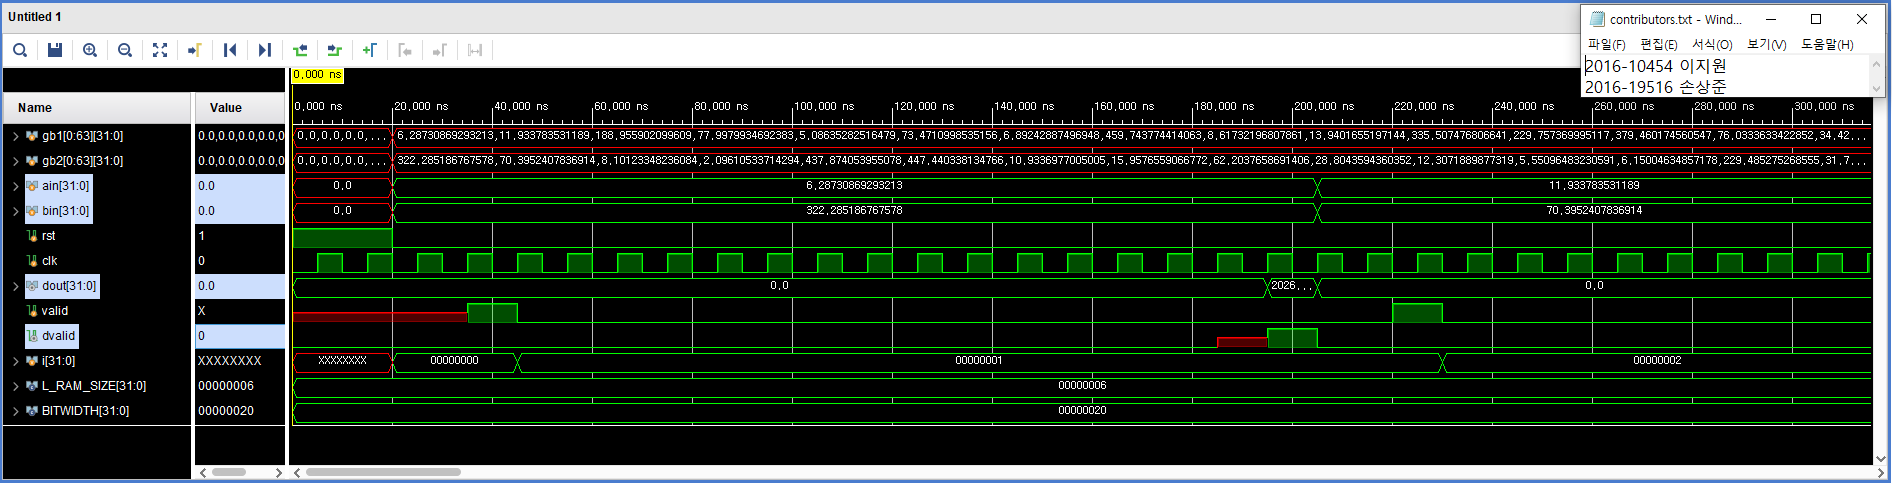
\includegraphics[width=1.0\textwidth]{../../submission/MY_PE/MY_PE_Waveform1.png}
	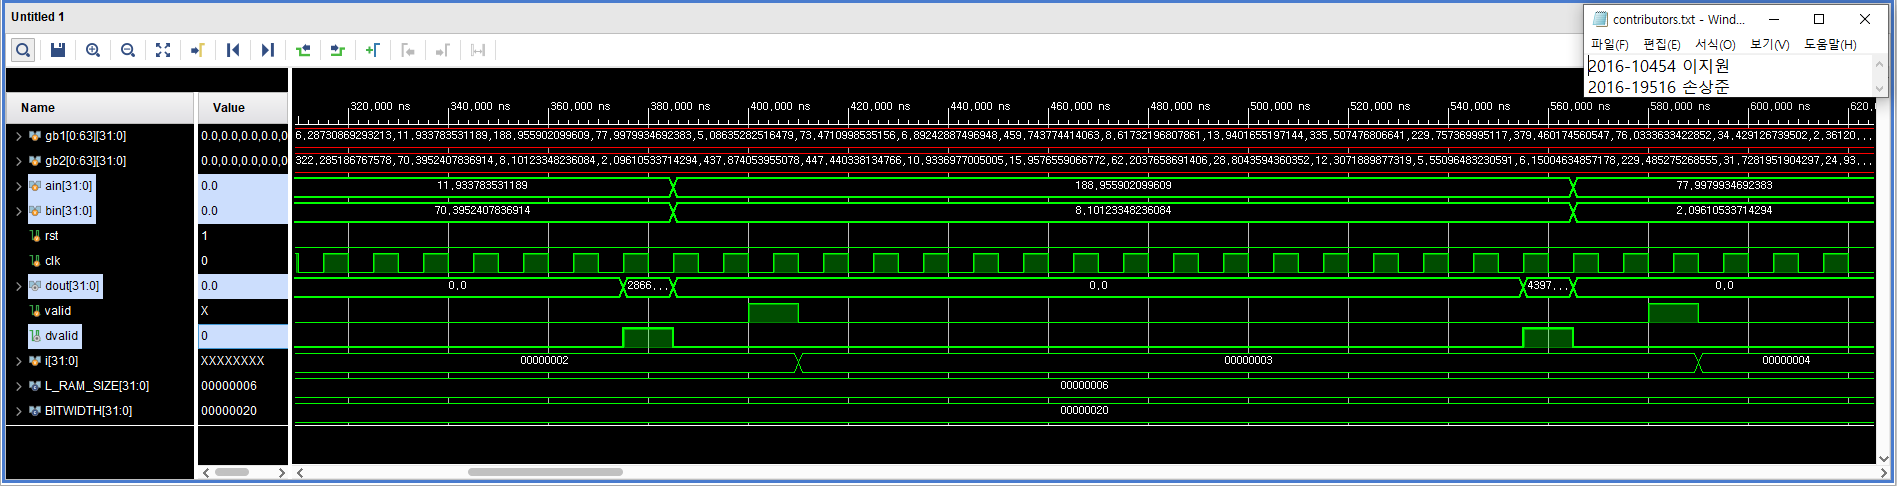
\includegraphics[width=1.0\textwidth]{../../submission/MY_PE/MY_PE_Waveform2.png}
\caption{\texttt{TB\_MY\_PE} Waveform}
\label{fig3}
\end{figure}

\section{Conclusion}

이후 프로젝트에서 어떤 모듈을 구현해야 하는지 Bottom-up으로 구현하다 보니 무슨 기능을 위한 구현인지는 아직 잘 모르겠지만 반대로 이전 lab 세션에서 구현을 진행한 모듈에 대해서는 연계성을 확인할 수 있었다. 지금 구현한 모듈이 앞으로도 쓰일 수 있기 때문에 가독성을 높이면서 최대한 임의 구현 방식을 최대한 피하기 위해 노력하였다. \\

MY\_BRAM 모듈을 구현하면서 WE signal에 따라 \texttt{mem}에 저장하는 statement를 for-generate로 구현해보려 했으나 이런 저런 오류가 나면서 나열형 방식으로 구현해 코드의 효율성이 떨어진다는 나름의 판단을 하였다. 추후 프로젝트를 진행하기 전에 always 구문 안에서 block assignment를 for-generate로 구현하는 방식을 익혀야 겠다는 필요성을 제고하였다~\cite{thomas2008verilog}.\\

MY\_PE 모듈 자체의 구현은 그리 어렵지 않았지만, IP catalog의 floating point MAC모듈의 내부 구조를 모르기 때문에, testbench를 작성하는데 어려움을 겪었는데, 이는 valid bit의 high 설정 후 dvalid bit가 high가 될 때까지의 정확한 clock cycle delay, valid bit와 input parameter가 동시에 할당되었을 때의 비정상적인 출력이 그리 직관적이지는 않았기 때문이라고 생각한다. MY\_PE 모듈도 이후 구현에서 중요한 부분을 차지하기 때문에, 최대한 이번 과제에만 국한되지 않게 구현하려 하였다. 

\bibliographystyle{plain}
\bibliography{other}

\end{document}
